\documentclass[12pt, titlepage]{article}

\usepackage{float}
\usepackage{booktabs}
\usepackage{tabularx}
\usepackage{hyperref}
\hypersetup{
    colorlinks,
    citecolor=black,
    filecolor=black,
    linkcolor=red,
    urlcolor=blue
}
\usepackage[round]{natbib}

\input{../Comments}
\input{../Common}

\begin{document}

\title{Verification and Validation Report: \progname} 
\author{\authname}
\date{\today}
	
\maketitle

\pagenumbering{roman}

\section{Revision History}

\begin{tabularx}{\textwidth}{p{3cm}p{2cm}X}
\toprule {\bf Date} & {\bf Version} & {\bf Notes}\\
\midrule
Date 1 & 1.0 & Notes\\
Date 2 & 1.1 & Notes\\
\bottomrule
\end{tabularx}

~\newpage

\section{Symbols, Abbreviations and Acronyms}

\renewcommand{\arraystretch}{1.2}
\begin{tabular}{l l} 
  \toprule		
  \textbf{symbol} & \textbf{description}\\
  \midrule 
  T & Test\\
  \bottomrule
\end{tabular}\\

\wss{symbols, abbreviations or acronyms -- you can reference the SRS tables if needed}

\newpage

\tableofcontents

\listoftables %if appropriate

\listoffigures %if appropriate

\newpage

\pagenumbering{arabic}

This document ...

\section{Functional Requirements Evaluation} \label{section:3} 

\subsection{Add a document to the database} \label{section:3.1}

This subsection covers FR1, FR4, and FR8 from of the \href{https://github.com/Inreet-Kaur/capstone/blob/main/docs/SRS/SRS.pdf}{SRS document} by testing that the system is able to add a document to the database only when a valid input is provided.

\begin{enumerate}

  \item{test-FR1,4,8-1} \label{test-FR1,4,8-1}
  
  Initial State: The system is set up, open to the following sections: Patient Records, Healthcare Professional Records and Healthcare Network Records. The system is ready to take the user input.

  Input: Correct and complete input data for all required fields.

  Expected Output: A confirmation message and a new entry is added to the appropriate database.

  Actual Output: A confirmation message and a new entry is added to the appropriate database.

  Result: Pass


  \item{test-FR1,4,8-2} \label{test-FR1,4,8-2}

  Initial State: The system is set up, open to the following sections: Patient Records, Healthcare Professional Records and Healthcare Network Records. The system is ready to take the user input.

  Input: Invalid input data.

  Expected Output: An error message outlining the invalid fields along with a possible steps to guide the users to recover from the error state.

  Actual Output: An error message outlining the invalid fields along with a possible steps to guide the users to recover from the error state.

  Result: Pass

\end{enumerate}

\subsection{Remove a document to the database} \label{section:3.2}

This subsection covers FR2, FR5, and FR9 from of the \href{https://github.com/Inreet-Kaur/capstone/blob/main/docs/SRS/SRS.pdf}{SRS document} by testing that the system is able to remove a document to the database only when a valid input idetifier is provided.

\begin{enumerate}

  \item{test-FR2,5,9-1} \label{test-FR2,5,9-1}
  
  Initial State: The system is set up, open to the following sections: Patient Records, Healthcare Professional Records and Healthcare Network Records. The system is ready to take the user input. A document exists in the appropriate database.

  Input: A correct identifier for the document to be deleted.

  Expected Output: A confirmation message and relevant entry no longer exist in the database.

  Actual Output: A confirmation message and relevant entry no longer exist in the database.

  Result: Pass


  \item{test-FR2,5,9-2} \label{test-FR2,5,9-2}

  Initial State: The system is set up, open to the following sections: Patient Records, Healthcare Professional Records and Healthcare Network Records. The system is ready to take the user input. A document exists in the appropriate database.

  Input: An invalid identifier for the document to be deleted.

  Expected Output: An error message outlining the invalid input along with a possible steps to guide the users to recover from the error state.

  Actual Output: An error message outlining the invalid input along with a possible steps to guide the users to recover from the error state.

  Result: Pass

\end{enumerate}

\subsection{Update a document to the database} \label{section:3.3}

This subsection covers FR3, FR6, FR10, and FR11 from of the \href{https://github.com/Inreet-Kaur/capstone/blob/main/docs/SRS/SRS.pdf}{SRS document} by testing that the system is able to update a document to the database only when a valid input idetifier is provided.

\begin{enumerate}

  \item{test-FR3,6,10,11-1} \label{test-FR3,6,10,11-1}
  
  Initial State: The system is set up, open to the following sections: Patient Records, Healthcare Professional Records and Healthcare Network Records. The system is ready to take the user input.

  Input: A correct identifier for the document to be updated.

  Expected Output: A confirmation message and relevant entry shows the updated data in the database.

  Actual Output: A confirmation message and relevant entry shows the updated data in the database.

  Result: Pass


  \item{test-FR3,6,10,11-2} \label{test-FR3,6,10,11-2}

  Initial State: The system is set up, open to the following sections: Patient Records, Healthcare Professional Records and Healthcare Network Records. The system is ready to take the user input.

  Input: An invalid identifier for the document to be updated.

  Expected Output: An error message outlining the invalid input along with a possible steps to guide the users to recover from the error state.

  Actual Output: An error message outlining the invalid input along with a possible steps to guide the users to recover from the error state.

  Result: Pass

\end{enumerate}

\subsection{Login for valid/invalid credentials} \label{section:3.4}

This subsection covers FR7 from of the \href{https://github.com/Inreet-Kaur/capstone/blob/main/docs/SRS/SRS.pdf} {SRS document} by testing that the system is able to allow to access the database only when a valid input credentials is provided.

\begin{enumerate}

  \item{test-FR7-1} \label{test-FR7-1}
  
  Initial State: The system is set up, open to the following sections: Patient Records, Healthcare Professional Records and Healthcare Network Records. The system is ready to take the user input.

  Input: The correct credentials for login.

  Expected Output: A confirmation message and user can access the homepage of the database.

  Actual Output: A confirmation message and user can access the homepage of the database.

  Result: Pass


  \item{test-FR7-2} \label{test-FR7-2}

  Initial State: The system is set up, open to the following sections: Patient Records, Healthcare Professional Records and Healthcare Network Records. The system is ready to take the user input.

  Input: Invalid credentials for login.

  Expected Output: An error message outlining the invalid fields.

  Actual Output: An error message outlining the invalid fields.

  Result: Pass

\end{enumerate}

\subsection{Voice-to-text-transcription check} \label{section:3.5}

This subsection covers FR7 from of the \href{https://github.com/Inreet-Kaur/capstone/blob/main/docs/SRS/SRS.pdf} {SRS document} by testing that the system is able to transcribe audio data to the written text.

\begin{enumerate}

  \item{test-FR11-1} \label{test-FR11-1}
  
  Initial State: The system is set up, open to the following sections: Patient Records, Healthcare Professional Records and Healthcare Network Records. The system is ready to take the user input.

  Input: A valid audio chunk from the conversation between the healthcare professional and the patient.

  Expected Output: A confirmation message indicating successful transcription and the screen shows the transcribed text.

  Actual Output: A confirmation message indicating successful transcription and the screen shows the transcribed text.

  Result: Pass


  \item{test-FR11-2} \label{test-FR11-2}

  Initial State: The system is set up, open to the following sections: Patient Records, Healthcare Professional Records and Healthcare Network Records. The system is ready to take the user input.

  Input: An invalid data format for transcription.

  Expected Output: An error message saying that the file or data format is not valid.

  Actual Output: An error message saying that the file or data format is not valid.

  Result: Pass

\end{enumerate}

\subsection{Validate output of correct diagnosis and medication} \label{section:3.6}

This subsection covers FR12 and FR13 from of the \href{https://github.com/Inreet-Kaur/capstone/blob/main/docs/SRS/SRS.pdf} {SRS document} by testing that the system is able to create predictions on the diagnosis and medicines with a high accuracy and confidence.

\begin{enumerate}

  \item{test-FR12,13-1} \label{test-FR12,13-1}
  
  Initial State: The user has uploaded the blank chart, and the chart has been populated with the patients symptoms.

  Input: Correct and complete input data where all the symptoms fields of the chart are filled out.

  Expected Output: A suggestion on what the diagnosis should be based on the symptoms, then based on the diagnosis provide possible medicine.

  Actual Output: A suggestion on what the diagnosis should be based on the symptoms, then based on the diagnosis provide possible medicine.

  Result: Pass

\end{enumerate}


\subsection{Validate input data for models} \label{section:3.7}

This subsection covers FR12, FR13, and IR5 from of the \href{https://github.com/Inreet-Kaur/capstone/blob/main/docs/SRS/SRS.pdf} {SRS document} by testing that the system is able to validate the input data in the charts such that it may be inputted into the prediction module.

\begin{enumerate}

  \item{test-FR12,13,IR5-1} \label{test-FR12,13,IR5-1}
  
  Initial State: The user has uploaded a blank chart.

  Input: Correct and complete input data where all the symptoms fields of the chart are filled out.

  Expected Output: A suggestion on what the diagnosis should be based on the symptoms, then based on the diagnosis provide possible medicine.

  Actual Output: A suggestion on what the diagnosis should be based on the symptoms, then based on the diagnosis provide possible medicine.

  Result: Pass

  \item{test-FR12,13,IR5-2} \label{test-FR12,13,IR5-2}
  
  Initial State: The user has uploaded the blank chart a blank chart.

  Input: Incorrect and incomplete input data where all the symptoms fields of the chart are filled out.

  Expected Output: An error message asking to fix the respective fields.

  Actual Output: An error message asking to fix the respective fields.

  Result: Pass

\end{enumerate}

\section{Nonfunctional Requirements Evaluation} \label{section:4}

\subsection{Aesthetic and Design} \label{section:4.1}

\begin{itemize}
\item \textbf{test-AD1} \label{test-AD1} \\
\textbf{Initial State:} UI is designed and implemented. \\
\textbf{Input:} Team members and peers view the UI under normal operating conditions. \\
\textbf{Output:} Feedback collected on UI’s aesthetic appeal and simplicity. \\
\textbf{Result:} Pass \\

\item \textbf{test-AD2} \label{test-AD2} \\
\textbf{Initial State:} UI is operational and accessible to users. \\
\textbf{Input:} Users interact with the UI during routine tasks and provide feedback. \\
\textbf{Output:} Team members and peers report satisfaction with the UI design. \\
\textbf{Result:} Pass \\
\end{itemize}

\subsection{Usability} \label{section:4.2}

\begin{itemize}
\item \textbf{test-UR1} \label{test-UR1} \\
\textbf{Initial State:} System is fully available and accessible to users after a 30-minute training session. \\
\textbf{Input:} Users perform key functions (logging in, accessing records, adding entries, generating reports). \\
\textbf{Output:} Team members and peers complete tasks without assistance within 2 minutes per task. \\
\textbf{Result:} Pass \\

\item \textbf{test-UR2} \label{test-UR2} \\
\textbf{Initial State:} System is deployed and accessible. \\
\textbf{Input:} Users navigate and explore system features independently. \\
\textbf{Output:} Majority of users can locate core functions without additional guidance. \\
\textbf{Result:} Pass \\
\end{itemize}

\subsection{Performance} \label{section:4.3}

\begin{itemize}
\item \textbf{test-PR1} \label{test-PR1} \\
\textbf{Initial State:} Transcription interface open and ready. \\
\textbf{Input:} Real-time voice input provided by healthcare professionals. \\
\textbf{Output:} Real-time transcription displayed within a 2-second delay. \\
\textbf{Result:} Pass \\
\end{itemize}

\subsection{Operational} \label{section:4.4}

\begin{itemize}
\item \textbf{test-OR1} \label{test-OR1} \\
\textbf{Initial State:} System is live and connected to monitoring software. \\
\textbf{Input:} 7-day operational period with intermittent load testing. \\
\textbf{Output:} Team members and peers monitored uptime consistently maintained at 99.9\% or above. \\
\textbf{Result:} Pass \\

\item \textbf{test-OR2} \label{test-OR2} \\
\textbf{Initial State:} System in operational use. \\
\textbf{Input:} Users access the system over a 7-day period under normal and peak loads. \\
\textbf{Output:} Team members and peers confirm that uptime meets standards without significant interruptions. \\
\textbf{Result:} Pass \\
\end{itemize}

\subsection{Maintainability} \label{section:4.5}

\begin{itemize}
\item \textbf{test-MR1} \label{test-MR1} \\
\textbf{Initial State:} System running on the latest version with recent update logs. \\
\textbf{Input:} Regular software update applied for bug fixes and improvements. \\
\textbf{Output:} System successfully applies updates without impacting stability. \\
\textbf{Result:} Pass \\

\item \textbf{test-MR2} \label{test-MR2} \\
\textbf{Initial State:} Previous version of the system with identified bugs or issues. \\
\textbf{Input:} Apply updates addressing known issues. \\
\textbf{Output:} System functions as expected with resolved issues and no new errors introduced. \\
\textbf{Result:} Pass \\
\end{itemize}

\subsection{Security} \label{section:4.6}

\begin{itemize}
\item \textbf{test-SR1} \label{test-SR1} \\
\textbf{Initial State:} System with live patient data encryption protocols active. \\
\textbf{Input:} Security audit test performed on the system. \\
\textbf{Output:} No vulnerabilities detected; all data remains encrypted in transit and at rest. \\
\textbf{Result:} Pass \\

\item \textbf{test-SR2} \label{test-SR2} \\
\textbf{Initial State:} System fully operational with access logs enabled. \\
\textbf{Input:} Simulate unauthorized access attempts. \\
\textbf{Output:} Unauthorized attempts are blocked; access logs capture details. \\
\textbf{Result:} Pass \\
\end{itemize}

\subsection{Cultural} \label{section:4.7}

\begin{itemize}
\item \textbf{test-CR1} \label{test-CR1} \\
\textbf{Initial State:} System operational in default language (English). \\
\textbf{Input:} User selects an alternate language from the settings menu. \\
\textbf{Output:} System displays all content in the selected language without loss of functionality. \\
\textbf{Result:} Fail \\
\end{itemize}

\subsection{Legal} \label{section:4.8}

\begin{itemize}
\item \textbf{test-LR1} \label{test-LR1} \\
\textbf{Initial State:} System is fully functional and contains patient records. \\
\textbf{Input:} Conduct a compliance audit with PIPEDA and other relevant data protection standards. \\
\textbf{Output:} System passes all compliance checks with no exceptions. \\
\textbf{Result:} Pass \\

\item \textbf{test-LR2} \label{test-LR2} \\
\textbf{Initial State:} System storing and transmitting patient data over a network. \\
\textbf{Input:} Monitor data handling and transfer processes during operation. \\
\textbf{Output:} All patient data is handled in compliance with regulations, without any unauthorized access or data breaches. \\
\textbf{Result:} Pass \\
\end{itemize}

\subsection{Scalability} \label{section:4.9}

\begin{itemize}
\item \textbf{test-S1} \label{test-S1} \\
\textbf{Initial State:} System deployed on a test server environment capable of scaling horizontally. \\
\textbf{Input:} Simulate an increasing number of concurrent users. \\
\textbf{Output:} System maintains consistent performance and response times without degradation. \\
\textbf{Result:} Pass \\
\end{itemize}

\subsection{Tests for Safety and Security Requirements} \label{section:4.10}

\subsubsection{Access Requirements Tests (AC1)} \label{section:4.10.1}

\begin{itemize}
\item \textbf{test-AC1-1} \label{test-AC1-1} \\
\textbf{Initial State:} System deployed with authentication module enabled and test user accounts configured. \\
\textbf{Input:} Attempt to access protected resources with invalid credentials. \\
\textbf{Output:}
\begin{itemize}
\item System logs each failed attempt.
\item User receives failed to login notification.
\end{itemize}
\textbf{Result:} Pass \\

\item \textbf{test-AC1-2} \label{test-AC1-2} \\
\textbf{Initial State:} System operational with authentication logs enabled. \\
\textbf{Input:} Attempt to access system resources without authentication. \\
\textbf{Output:} 
\begin{itemize}
    \item All unauthorized access attempts are blocked.
    \item Each attempt is logged with timestamp, IP address, and attempted resource.
\end{itemize}
\textbf{Result:} Pass \\
\end{itemize}

\subsubsection{Access Requirements Test (AC2)} \label{section:4.10.2}

\begin{itemize}
\item \textbf{test-AC2-1} \label{test-AC2-1} \\
\textbf{Initial State:} System operational with standard user and admin accounts configured. \\
\textbf{Input:} Attempt to create, update, and delete user accounts using non-admin credentials. \\
\textbf{Output:}
\begin{itemize}
\item All unauthorized actions are blocked.
\item Actions are logged with user details.
\item Security team can review blocked attempts.
\end{itemize}
\textbf{Result:} Pass \\
\end{itemize}

\subsubsection{Integrity Requirements Tests (IR1)} \label{section:4.10.3}

\begin{itemize}
\item \textbf{test-IR1-1} \label{test-IR1-1} \\
\textbf{Initial State:} System operational with test user accounts and authentication database. \\
\textbf{Input:} Simulate multiple concurrent failed login attempts while monitoring credential storage. \\
\textbf{Output:} User credentials remain unchanged, and system maintains stability. \\
\textbf{Result:} Pass \\
\end{itemize}

\subsubsection{Integrity Requirements Tests (IR2)} \label{section:4.10.4}

\begin{itemize}
\item \textbf{test-IR2-1} \label{test-IR2-1} \\
\textbf{Initial State:} System is set up, open to the relevant section, and ready to take user input. \\
\textbf{Input:} Submit an invalid data input. \\
\textbf{Output:} An error message is displayed to the user. No data is added to any database. \\
\textbf{Result:} Pass \\
\end{itemize}

\subsubsection{Integrity Requirements Tests (IR3)} \label{section:4.10.5}

\begin{itemize}
\item \textbf{test-IR3-1} \label{test-IR3-1} \\
\textbf{Initial State:} The prediction model is ready to predict medication and diagnosis. \\
\textbf{Input:} A test set of various patient medical charts. \\
\textbf{Output:} The prediction includes a diagnosis and medication prediction, each with a confidence score exceeding 85\%. \\
\textbf{Result:} Pass \\
\end{itemize}

\subsubsection{Integrity Requirements Tests (IR4)} \label{section:4.10.6}

\begin{itemize}
\item \textbf{test-IR4-1} \label{test-IR4-1} \\
\textbf{Initial State:} System is set up, open to the relevant section, and ready to take user input. A document already exists in the relevant database. \\
\textbf{Input:} A new input with the same data as an existing document. \\
\textbf{Output:} An error message is displayed. No new document is added to the database. \\
\textbf{Result:} Pass \\
\end{itemize}

\subsubsection{Integrity Requirements Tests (IR5)} \label{section:4.10.7}

\begin{itemize}
\item \textbf{test-IR5-1} \label{test-IR5-1} \\
\textbf{Initial State:} System is set up, open to the relevant section, and ready to take user input. A document already exists in the relevant database. \\
\textbf{Input:} Written text transcribed from the audio data. \\
\textbf{Output:} The data is correctly classified in the generated report with no diagnosis errors. \\
\textbf{Result:} Pass \\
\end{itemize}

\subsubsection{Integrity Requirements Tests (IR6)} \label{section:4.10.8}

\begin{itemize}
\item \textbf{test-IR6-1} \label{test-IR6-1} \\
\textbf{Initial State:} System is set up, open to the relevant section, and ready to take user input. \\
\textbf{Input:} Audio conversation between the patient and healthcare professional. \\
\textbf{Output:} The written text transcribed from the input data matches the conversation with minimal to no interference. \\
\textbf{Result:} Pass \\
\end{itemize}


\section{Comparison to Existing Implementation}	

This section will not be appropriate for every project.

\section{Unit Testing}

\subsection{Behaviour-Hiding Module}

\subsubsection{User Authentication Module}

\begin{enumerate}

  \textbf{Control:} Manual

  \textbf{Initial State:} The default email and password are initialized as variables and given a default value.

  \textbf{Test Case Derivation:} The expected behavior is derived from the correct registration and login functionality of Firebase Authentication, ensuring valid user creation and authentication processes, as well as error handling for invalid credentials.

  \textbf{Test Procedure:} The tests are performed as follows:

  \begin{itemize}
    \item Sign up using valid credentials:

    \begin{itemize}
      \item \textbf{Input:} The input for this test are the valid credentials of email and password.
      \item \textbf{Output:} The user object is returned by the signup function.
      \item \textbf{Test Derivation:} Verifies that the signup function correctly works and creates a new user account when the valid credentials are provided.
    \end{itemize}

    \item Sign up throwing errors with invalid credentials:

    \begin{itemize}
      \item \textbf{Input:} The input for this test are the invalid credentials of email and password.
      \item \textbf{Output:} An error thrown up by the signup function.
      \item \textbf{Test Derivation:} Verifies that the signup function correctly throws error when the invalid credentials are provided.
    \end{itemize}

    \item Sign in using valid credentials:

    \begin{itemize}
      \item \textbf{Input:} The input for this test are the valid credentials of email and password. 
      \item \textbf{Output:} The user object is returned by the signin function.
      \item \textbf{Test Derivation:}  Verifies that the signin function correctly authenticates the user when valid credentials are provided.
    \end{itemize}

    \item Sign in throwing errors with invalid credentials: 

    \begin{itemize}
      \item \textbf{Input:} The input for this test are the invalid credentials of email and password. 
      \item \textbf{Output:} An error thrown up by the signin function.
      \item \textbf{Test Derivation:} Verifies that the signin function correctly throws error when the invalid credentials are provided.
    \end{itemize}
  \end{itemize}
\end{enumerate}











\section{Changes Due to Testing}

\wss{This section should highlight how feedback from the users and from 
the supervisor (when one exists) shaped the final product.  In particular 
the feedback from the Rev 0 demo to the supervisor (or to potential users) 
should be highlighted.}

\section{Automated Testing}
		
\section{Trace to Requirements}

\begin{table}[H]
  \centering
  \begin{tabular}{|c|c|c|c|c|c|c|c|c|c|c|c|c|c|c|}
  \hline
   Test ID & FR1 & FR2 & FR3 & FR4 & FR5 & FR6 & FR7 & FR8 & FR9 & FR10 & FR11 & FR12 & FR13 & FR14\\
  \hline
  test-FR1,4,8-\ref{test-FR1,4,8-1} & $\times$ & & & $\times$ & & & & $\times$ & & & & & & \\
  \hline
  test-FR1,4,8-\ref{test-FR1,4,8-2} & $\times$ & & & $\times$ & & & & $\times$ & & & & & & \\
  \hline
  test-FR2,5,9-\ref{test-FR2,5,9-1} & & $\times$ & & & $\times$ & & & & $\times$ & & & & & \\
  \hline
  test-FR2,5,9-\ref{test-FR2,5,9-2} & & $\times$ & & & $\times$ & & & & $\times$ & & & & & \\
  \hline
  test-FR3,6,10,11-\ref{test-FR3,6,10,11-1} & & & $\times$ & & & $\times$ & & & & $\times$ & $\times$ & & & \\
  \hline
  test-FR3,6,10,11-\ref{test-FR3,6,10,11-2} & & & $\times$ & & & $\times$ & & & & $\times$ & $\times$ & & & \\
  \hline
  test-FR7-\ref{test-FR7-1} & & & & & & & $\times$ & & & & & & & \\
  \hline
  test-FR7-\ref{test-FR7-2} & & & & & & & $\times$ & & & & & & & \\
  \hline
  test-FR11-\ref{test-FR11-1} & & & & & & & & & & & $\times$ & & & \\
  \hline
  test-FR11-\ref{test-FR11-2} & & & & & & & & & & & $\times$ & & & \\
  \hline
  test-FR12,13-\ref{test-FR12,13-1} & & & & & & & & & & & & $\times$ & $\times$ & \\
  \hline
  test-FR12,13,IR5-\ref{test-FR12,13,IR5-1} & & & & & & & & & & & & $\times$ & $\times$ & \\
  \hline
  test-FR12,13,IR5-\ref{test-FR12,13,IR5-2} & & & & & & & & & & & & $\times$ & $\times$ & \\
  \hline
  test-FR14-\ref{test-FR14-1} & & & & & & & & & & & & & & $\times$ \\
  \hline
\end{tabular}
\caption{\bf Functional Requirements Tests Traceability} \label{tab:fr-test-traceability}
\end{table}


\begin{table} [H]
  \centering
  \begin{tabular}{|c|c|c|c|c|c|c|c|c|c|}
    \hline
    TestID & NFR1 & NFR2 & NFR3 & NFR4 & NFR5 & NFR6 & NFR7 & NFR8 & NFR9 \\
    \hline
    test-AD\ref{test-AD1} & $\times$ & & & & & & & & \\
    \hline
    test-AD\ref{test-AD2} &  $\times$ & & & & & & & & \\
    \hline
    test-UR\ref{test-UR1} & & $\times$ &  & & & & & & \\
    \hline
    test-UR\ref{test-UR2} & & $\times$ & & & & & & &  \\
    \hline
    test-PR\ref{test-PR1} & & & $\times$ & & & & & & \\
    \hline
    test-OR\ref{test-OR1} & & & & $\times$ & & & & &  \\
    \hline
    test-OR\ref{test-OR2} & & & & $\times$ & & & & & \\
    \hline
    test-MR\ref{test-MR1} & & & & & $\times$ & & & &\\
    \hline
    test-MR\ref{test-MR2} & & & & & $\times$ & & & &  \\
    \hline
    test-SR\ref{test-SR1} & & & & & & $\times$ & & &\\
    \hline
    test-SR\ref{test-SR2} & & & & & & $\times$ & & & \\
    \hline
    test-CR\ref{test-CR1} & & & & & & & $\times$ & &\\
    \hline
    test-LR\ref{test-LR1} & & & & & & & & $\times$ &\\
    \hline
    test-LR\ref{test-LR2} & & & & & & & & $\times$ & \\
    \hline
    test-S\ref{test-S1} & & & & & & & & & $\times$ \\
    \hline
  \end{tabular}
\caption{\bf Non-Functional Requirements Tests Traceability} \label{tab:nfr-test-traceability}
\end{table}

\begin{table} [H]
  \centering
  \begin{tabular}{|c|c|c|c|c|c|c|c|c|c|}
  \hline
  Test ID & AC1 & AC2 & IR1 & IR2 & IR3 & IR4 & IR5 & IR6 \\
  \hline
  test-AC1-\ref{test-AC1-1} & $\times$ & & & & & & &   \\
  \hline
  test-AC1-\ref{test-AC1-2} & $\times$ & & & & & & &   \\
  \hline
  test-AC2-\ref{test-AC2-1} & & $\times$ & & & & & &   \\
  \hline
  test-IR1-\ref{test-IR1-1} & & & $\times$ & & & & &   \\
  \hline
  test-IR2-\ref{test-IR2-1}  & & & & $\times$ & & & &  \\
  \hline
  test-IR3-\ref{test-IR3-1}  & & & & & $\times$ & & &  \\
  \hline
  test-IR4-\ref{test-IR4-1}  & & & & & & $\times$ & &  \\
  \hline
  test-IR5-\ref{test-IR5-1}  & & & & & & &  $\times$ & \\
  \hline
  test-IR6-\ref{test-IR6-1}  & & & & & & & &  $\times$ \\
  \hline
\end{tabular}
\caption{\bf Safety and Security Requirements Tests Traceability} \label{tab:sns-test-traceability}
\end{table}
		
\section{Trace to Modules}		

\section{Code Coverage Metrics}

The image below displays the code coverage metrix. This includes all the files, includes the files for which the team created unit tests. Although some files such as firebase.ts and DatabaseOps.ts for which we have developed the unit tests demonstrate higher test coverage, the overall test coverage is lower. This is because most of the code is prewritten which is why only 55.06'\%' and 30.12'\%' of branches are covered as per the metrcs. The figure below show the code coverage metrics example for RapidCare.

\begin{figure}[h]
  \centering
  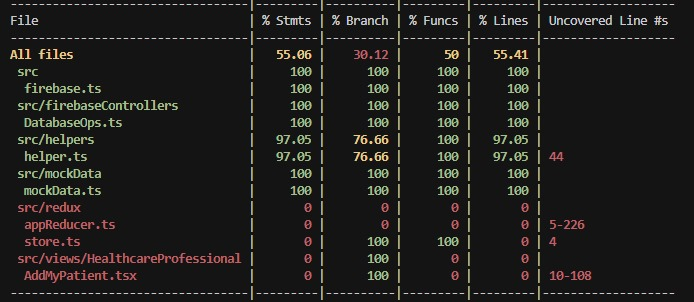
\includegraphics[width=1\textwidth]{code_coverage_metrics.jpg}
  \caption{Code Coverage Metrics}
\end{figure}

\bibliographystyle{plainnat}
\bibliography{../../refs/References}

\newpage{}
\section*{Appendix --- Reflection}

The information in this section will be used to evaluate the team members on the
graduate attribute of Reflection.

\input{../Reflection.tex}

\begin{enumerate}
  \item What went well while writing this deliverable?
  This document has let us strengthen the understanding about unit testing of all functional requirements as well as verification of all non-functional qualities of the system. While going through the outline of the document, we were able to conduct unit testing and compare it with the existing implementation. It also made us better execute the detailed procedure of system testing along with performing validation and verification of the system. 

  \item What pain points did you experience during this deliverable, and how did you resolve them?
  There are obstacles in any team project that must be overcome for it to proceed successfully. To ensure seamless operations, we had to develop a strategy for contributions. Since we already had the list of tests that were needed to be conducted for both functional and non-functional requirements, we divided them equally among all the team members. We also needed to create a schedule to contribute to the template and review each other's work in the best way possible. 

  \item Which parts of this document stemmed from speaking to your client(s) or a proxy (e.g. your peers)? Which ones were not, and why?
  The client's feedback helped us to understand the changes due to testing the requirements. Before Rev 0 demo, the team gave a demo to the supervisor about the system pretending the supervisor as the healthcare professional using the system. The supervisor then gave us some possible ways that the healthcare professional would like to use the system. This helped us to improve some features of the system such as whether prescription of a patient is being saved or not. If yes, then is it being stored within the system or on local machine. Furthermore, the section such as unit testing of all functional requirements stemmed from the collective ideas of our peers. We discussed different test cases that each requirement could possibly have along with how they will be implemented. In this way, we got diverse test cases and all team members were able to contribute especially in this critical section of the report.

  \item In what ways was the Verification and Validation (VnV) Plan different
  from the activities that were actually conducted for VnV?  If there were
  differences, what changes required the modification in the plan?  Why did
  these changes occur?  Would you be able to anticipate these changes in future
  projects?  If there weren't any differences, how was your team able to clearly
  predict a feasible amount of effort and the right tasks needed to build the
  evidence that demonstrates the required quality?  (It is expected that most
  teams will have had to deviate from their original VnV Plan.)
  VnV Plan was little bit different from the activities that were actually conducted and recorded in VnV Report. This is because VnV Plan includes one extra functional requirement test which needs to be deleted as the team has decided to not pursue with that functional requirement. Therefore, the team will modify the VnV Plan to remove that requirement.Additionally, as part of the modifications, the team removed some Non-Functional Requirements tests to reduce redundancy, such as test-S2, test-CR2, and test-PR1, and updated the traceability to the requirements for both Non-Functional Requirements tests and Safety and Security tests. These changes were made to streamline the testing process and ensure alignment with the system's goals. This change occured as we went through every detail of our system and it turns out that functional requirement is not necessary for the system to accomplish its goal. Yes, we will be able to anticipate thus change in the future projects as going through every detail of the project review the necessary and non-necessary features of the product.  

\end{enumerate}

\end{document}